\subsection{Putting Together}
\label{sec:together}
\begin{figure}
	\centering
	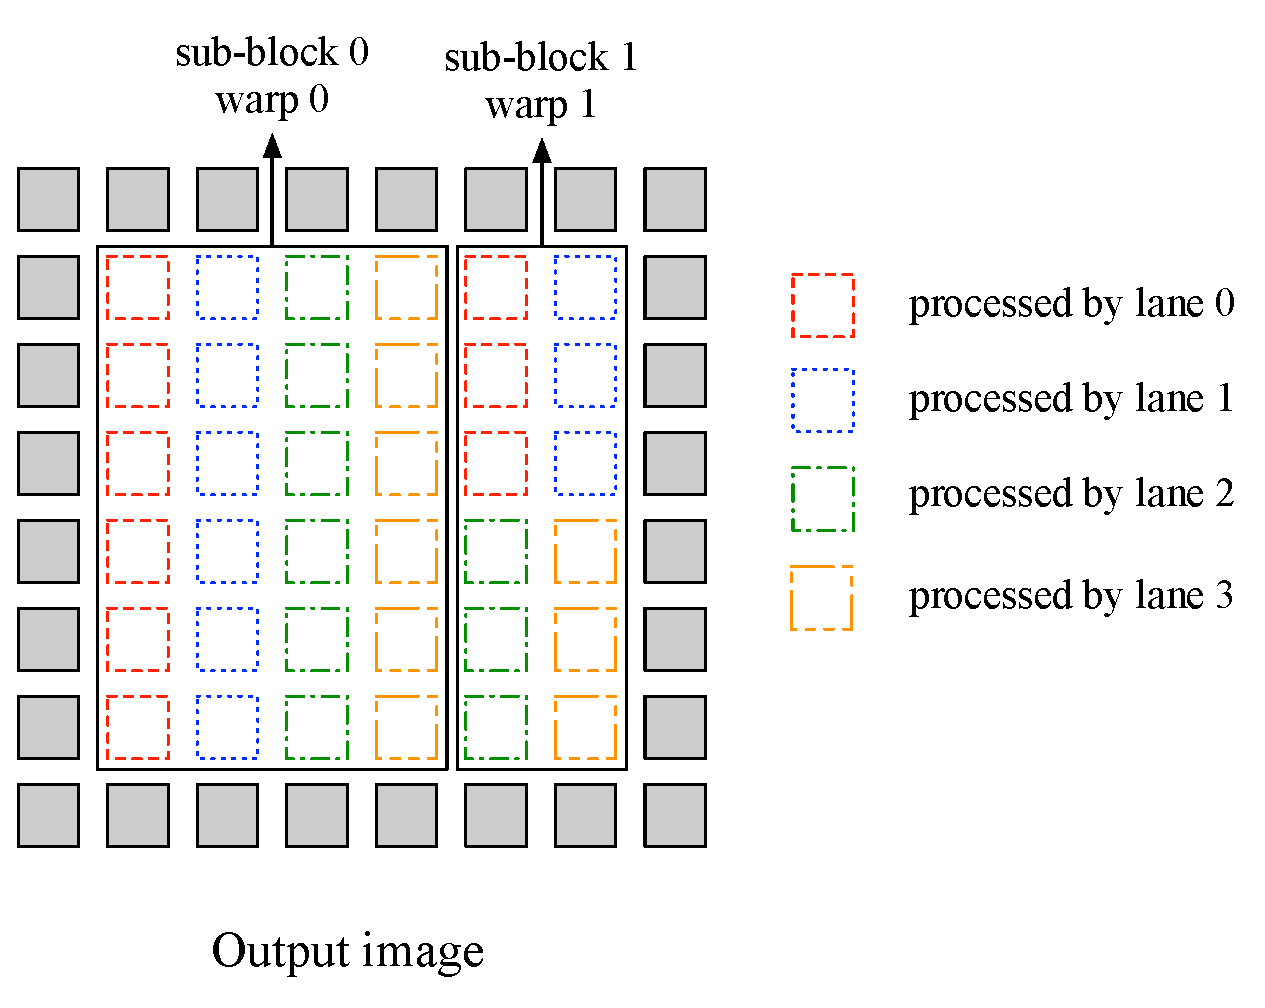
\includegraphics[width=0.8\columnwidth,height=5cm]{./figure/overalldesign.eps} 
	\vspace{-3mm}
	\caption{The output is produced by sliding a $3 \times
3$ filter over an $8 \times 8$ input with one pad. Here, we assume
that the warp size is 4 and thus having $laneid=threadid\%4$.} \label{fig:overalldesign}
\end{figure}


We have individually demonstrated how our column and row reuse optimizations can be used together to optimize GPU memory accesses for
depthwise convolution operations. We now take the widely used 2D convolution as an example to illustrate how to apply both reuse algorithms
on convolution operations.


To apply our approach to depthwise convolution that works on a 2D matrix, we first divide the output into sub-blocks. Each sub-block
contains exactly $n$ columns (in this work, $n = 32$, which is the default warp size of our GPU platform). The only exception is the last
sub-block, which may contain less than $n$ columns. If a sub-block contains more than $k$ rows ($k=56$ in this work), we then further
break down the sub-block along the height dimension. \RV{The blocking method implies that our approach can handle arbitrary input sizes}. Each GPU thread block will process one or multiple sub-blocks, and each warp will
compute one sub-block. As a result, the threads within the same warp will process the adjacent columns of one sub-block.


\begin{algorithm}[t!]
\small
	\KwIn{$I$, $F$, $subBlockHeight$}
	\KwOut{$O$}
	Load the filter into shared memory\;
	Divide columns of the filter into a combination of 3-column and 5-column sub-filters\;
	$\_\_syncthreads()$\;
	\If{$blockIdx.x \textless gridDim.x-1$}{
		Init thread local register array $sum$ to zero\;
		Calculate the index of the first input element this thread needs, denoted as $inputIndex$\;
		\For{$i \gets 0$ \KwTo $subBlockHeight$}{
			\ForEach{sub-filter}{
				Load corresponding input elements from $inputIndex$ of global memory into $iTemp$\;
				Call $RetrieveThirdElement(iTemp)$ or $RetrieveSecondElement(iTemp)$\;
				Call $RowReuse(iTemp,i,$\textit{sub-filter}$,sum)$\;
			}
			Write completed element of $sum$ into $O$\;
		}		
		
	}
	\Else{
		Divide columns of the last sub-block into multiple partitions and try to evenly assign those partitions to threads of a warp. Each thread uses a direct method to calculate elements of $O$.\;
		The same method is adopted when processing the edge elements of $O$\;
	}
	\caption{Depthwise Convolution}
	\label{algo:overalldesign}
\end{algorithm}

\subsubsection{Example} Fig. \ref{fig:overalldesign} shows the mapping process of GPU threads to output elements. In this example, we slide a $3
\times 3$ filter over an $8 \times 8$ input. To apply a square  filter at the edge of the image, we need to pad the input. To reduce the
memory pressure, we do not allocate GPU memory space for the padded elements. Instead, we use different methods to calculate the edge and
inner elements of the output. The edge and inner elements are represented by the shaded and dashed squares in Fig.
\ref{fig:overalldesign}, respectively.


In this example, we assume each GPU warp contains four threads. Therefore, we will divide the inner elements into multiple sub-blocks and
each sub-block contains four columns so that a column can be processed by one of the four GPU threads within a wrap. In our case, we will
have two sub-blocks, where sub-block 0 contains four columns, but sub-block 1 only contains two columns. To utilize the threads within a
warp, we divide elements of the last two columns evenly among the four threads.

\subsubsection{Generalization} In Algorithm \ref{algo:overalldesign}, we describe our generalized solution. Here, we process the sub-blocks
with exactly 32 columns (i.e., the default wrap size of our evaluation GPU) and the last sub-block in Lines 4-15 and 16-19, respectively.
In this way, each GPU thread calculates one column of the output elements. This is done through several steps. First, each thread block
loads the filter into shared memory and divides the filter into a combination of 3-column and 5-column sub-filters. Next, each thread
calculates the address of the first input element it needs (Lines 6). For each output element and sub-filter, each thread loads
corresponding input elements into $iTemp$ and passes $iTemp$ to Algorithms \ref{algo:basic} and \ref{algo:basic2} to fill the row vector $iTemp$
(Line 10). Then, each thread passes the filled vector $iTemp$ to Algorithm \ref{algo:rowreuse} to calculate multiple output elements and
store results in the register array $sum$ (Line 11). Finally, when the calculation of one output element is completed, we write the
corresponding result in $sum$ into the result array $O$ (Line 13).
